\chapter{The Minimal Supersymmetric Model}
\label{chap:mssm}

In addition to the SU(3) $\times$ SU(2) $\times$ U(1) symmetry imposed on the Lagrangian within the Standard Model, one can introduce additional \textit{supersymmetrys} to the theory. Supersymmetry transformations act on fields containing both fermionic and bosonic degrees of freedom, the Lagrangian is required to remain invariant under rotations between these two states. Many such extensions to the Standard Model exist, but only the simplest of these, requiring a single global transformation $Q$, is phenomenologically viable: the Minimal Supersymmetric Standard Model (MSSM). In this theory, every Standard Model particle has a \textit{superpartner} which differs by 1/2 unit of spin but otherwise has identical properties. The most striking prediction of the MSSM is a doubling of the known particle content of the Universe. Table \ref{tab:mssmparticles} lists the supersymmetric partners to the Standard Model particles, the complement of Table \ref{tab:smparticles}. An additional spin-0 Higgs doublet, with neutral and negatively charged components, is required by the theory. Thus we do not expect only a neutral spin-1/2 superpartner for the Higgs boson, but in fa

This chapter is adapted from \cite{susyprimer}.

Matter particles (both the left and right-chiral components) are placed in \textit{chiral supermultiplets} consisting of a spin-1/2 Majorana fermion $\psi$ and complex scalar field $\phi$. In the massless and non-interacting case (i.e. just the two kinetic terms in the Lagrangian, known as the \textit{Wess-Zumino model} \cite{wesszumino}), the transformation laws of the fields can be deduced by demanding invariance under the simple Lagrangian, they are found to be:
 
\begin{equation}
\begin{array}{l}
\psi \xrightarrow[]{\text{Q}} \psi - i ( \sigma^{\mu} \epsilon^{\dagger} ) \partial_{\mu} \phi \\
\phi \xrightarrow[]{\text{Q}} \phi + \epsilon \psi \\
\end{array}
\end{equation}
where $\epsilon$ is a 2-component Weyl \textbf{spinor} parametrizing the transformation. For the duration of this chapter, all references to \textit{auxiliary} fields will be omitted. Auxiliary fields are internal to the theory and must be introduced to allow the fields to satisfy their classical wave equations.

Renormalizability restrict the numbers of fields in any interaction involving $\psi$ and $\phi$, the most generic Lagrangian for a chiral supermultiplet is of the form:

\begin{equation}
\label{eq:lchiral}
\mathcal{L}_{chiral} = - D^{\mu}\phi^{*}D{\mu}\phi - V(\phi, \phi^{*}) + i \psi^{\dagger}\bar{\sigma}^{\mu} D{\mu}\psi - \frac{1}{2} (M \psi \psi + h.c.) - \frac{1}{2} (y \phi  \psi \psi + h.c.)
\end{equation}
where $D^{\mu}$ is the covariant derivative, $V(\phi, \phi^{*})$ is a scalar potential for the theory, $\bar{\sigma}^{0}$ is the 2x2 identity matrix and $\bar{\sigma}^{123}\equiv-\sigma^{123}$, M is a (Majorana) mass term, $\psi\psi\equiv\epsilon^{ab}\psi_{a}\psi_{b}$, and $y$ is a Yukawa coupling.

The Yukawa coupling connects two SM fermions with its corresponding scalar field - the vertex for this process is seen in Figure \ref{fig:mssmfeyn}a. Additional interactions with the gauge bosons of the theory (SM $A^{a}_{\mu}$ to be discussed later) are introduced due to the action of the covariant derivative acting on the scalar field $\partial_{\mu} \phi \rightarrow \partial_{\mu}\phi -igA^{a}_{\mu}T^{a}\phi$. Expanding out this kinetic term, we find the following two interactions: $-ig[(\partial_{\mu}\phi)A^{a}_{\mu}T^{a}\phi+h.c.]$ and $g^{2}A^{a\mu}\phi^{*}t^{a}A^{a}_{\mu}T^{a}\phi$, seen in Figures \ref{fig:mssmfeyn}(d) and (e), respectively. Throughout this chapter I will focus on only on interactions involving at least one SM particle and at least one supersymmetric particle.

Gauge bosons (before spontaneous symmetry breaking) are placed in \textit{gauge supermultiplets} consisting of a gauge bosons A$^{\mu}_{a}$ and spin-1/2 gaugino $\lambda_{a}$; $a$ is a label which runs over the gauge SM gauge fields for the theory.

Under the supersymmetry, fields can be found to transform as:
\begin{equation}
\begin{array}{l}
A_{\mu}^{a} \xrightarrow[]{\text{Q}} A_{\mu}^{a} - \frac{1}{\sqrt{2}} ( \epsilon^{\dagger} \bar{\sigma}_{\mu} \lambda + h.c)\\
\lambda_{\alpha}^{a} \xrightarrow[]{\text{Q}} \lambda_{\alpha} + \frac{i}{2\sqrt{2}}(\sigma^{\mu}\bar{\sigma}^{\nu}\epsilon)F_{\mu\nu}^{a}
\end{array}
\end{equation}
where $F_{\mu\nu}^{a}$ is the regular field strength tensor for the gauge field $A_{\mu}^{a}$.

The SM symmetries (i.e. SU(3), SU(2), U(1)) transform the gauge supermultiplet in the following way:
\begin{equation}
\begin{array}{l}
A_{\mu}^{a} \xrightarrow[]{\text{SM}}  A_{\mu}^{a} + \partial_{\mu}\Lambda^{a} + gf^{ijk}A_{\mu}^{b}\Lambda^{c}\\
\lambda^{a} \xrightarrow[]{\text{SM}}  \lambda^{a} + gf^{abc}\lambda^{b}\Lambda^{c}
\end{array}
\end{equation}
where $\Lambda^{a}$ is a parameter describing the the transformation. The transformation law for $A^{\mu}$ is the usual and customary for gauge fields, as seen in Chapter \ref{chap:sm}.

The Lagrangian for a free gauge multiplet consists simply of the kinetic terms for each:
\begin{equation}
\mathcal{L}_{gauge} = -\frac{1}{4}F_{\mu\nu}F^{\mu\nu} + i \lambda^{\dagger}\bar{\sigma}^{\mu}\nabla\lambda^{a}
\end{equation}
where $f^{abc}$ are the structure constants of the gauge group. $\nabla\lambda^{a} = \partial_{\mu}\lambda^{a}+gf^{abc}A^{b}_{\mu}\lambda^{c}$ represents the covariant derivative acting on $\lambda^{a}$ - creating an interaction term between a gauge boson and two gauginos, as seen in Figure \ref{fig:mssmfeyn}c.

Renormalization restricts the interactions between the gauge and chiral supermultiplets to be only of the form $-\sqrt{2}g(\phi^{*}T^{a}\psi\lambda^{a}+h.c.)$, involving a single spin-0, spin-1/2, and spin-1 particle - the vertex is seen in Figure \ref{fig:mssmfeyn}(e).

\begin{figure}[hb!]
\centering
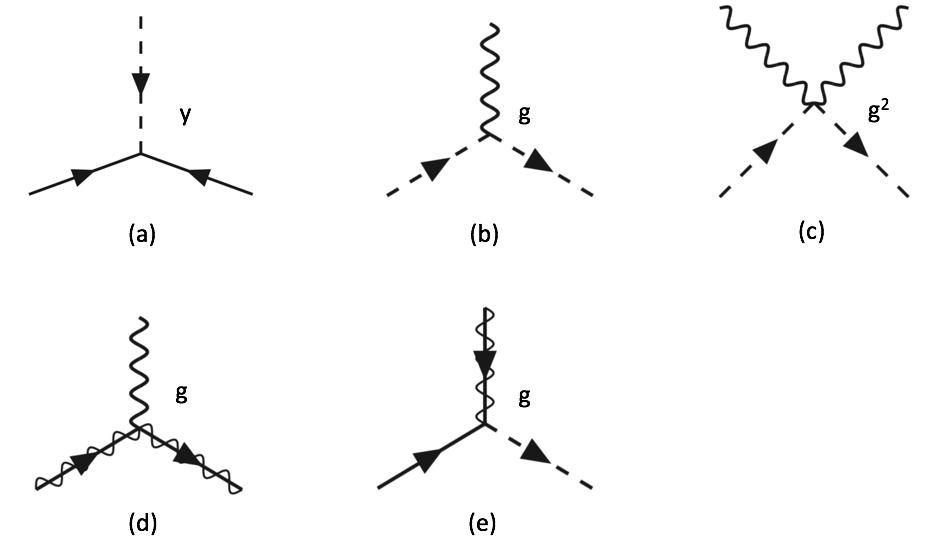
\includegraphics[width=0.75\textwidth]{figs/mssmfeyn.png}
\caption{Possible interactions between SM and supersymmetric particles. The strength of the interaction is labeled in the top right of each diagram.}
\label{fig:mssmfeyn}
\end{figure}

Within a supersymmetric theory, the superpartners are required to have the same mass as their corresponding SM field. If the masses of these particles were of the same scale as that seen in the SM we would have expected to see evidence of them over the years while the SM itself was being developed. There must be some mechanism which breaks the supersymmetry and generates large enough mass for the superpartners such that they could not have been detected over the years.

The focus of the remainder of these thesis is a search for evidence of physics beyond the Standard Model, such as theories as the MSSM. The motivation for our particular signal region is highly motivated by final state topologies arising from gluino pair production. The gluino is the spin-1/2 fermion which is the superpartner to the gluon, the mediator of the strong force. Within the context of QCD - the chiral supermultiplets consist of spin-1/2 quarks and spin-0 squarks. Searches for supersymmetric particles of QCD are partly motivated by the fact that most of their production mechanisms proceed through diagrams proportional to the strong coupling constant $g_{s}$, which is largest among the three in the Standard Model. The possible tree-level diagrams for gluino pair production are shown in Figure \ref{fig:gluinopair}.

\begin{figure}[hb!]
\centering
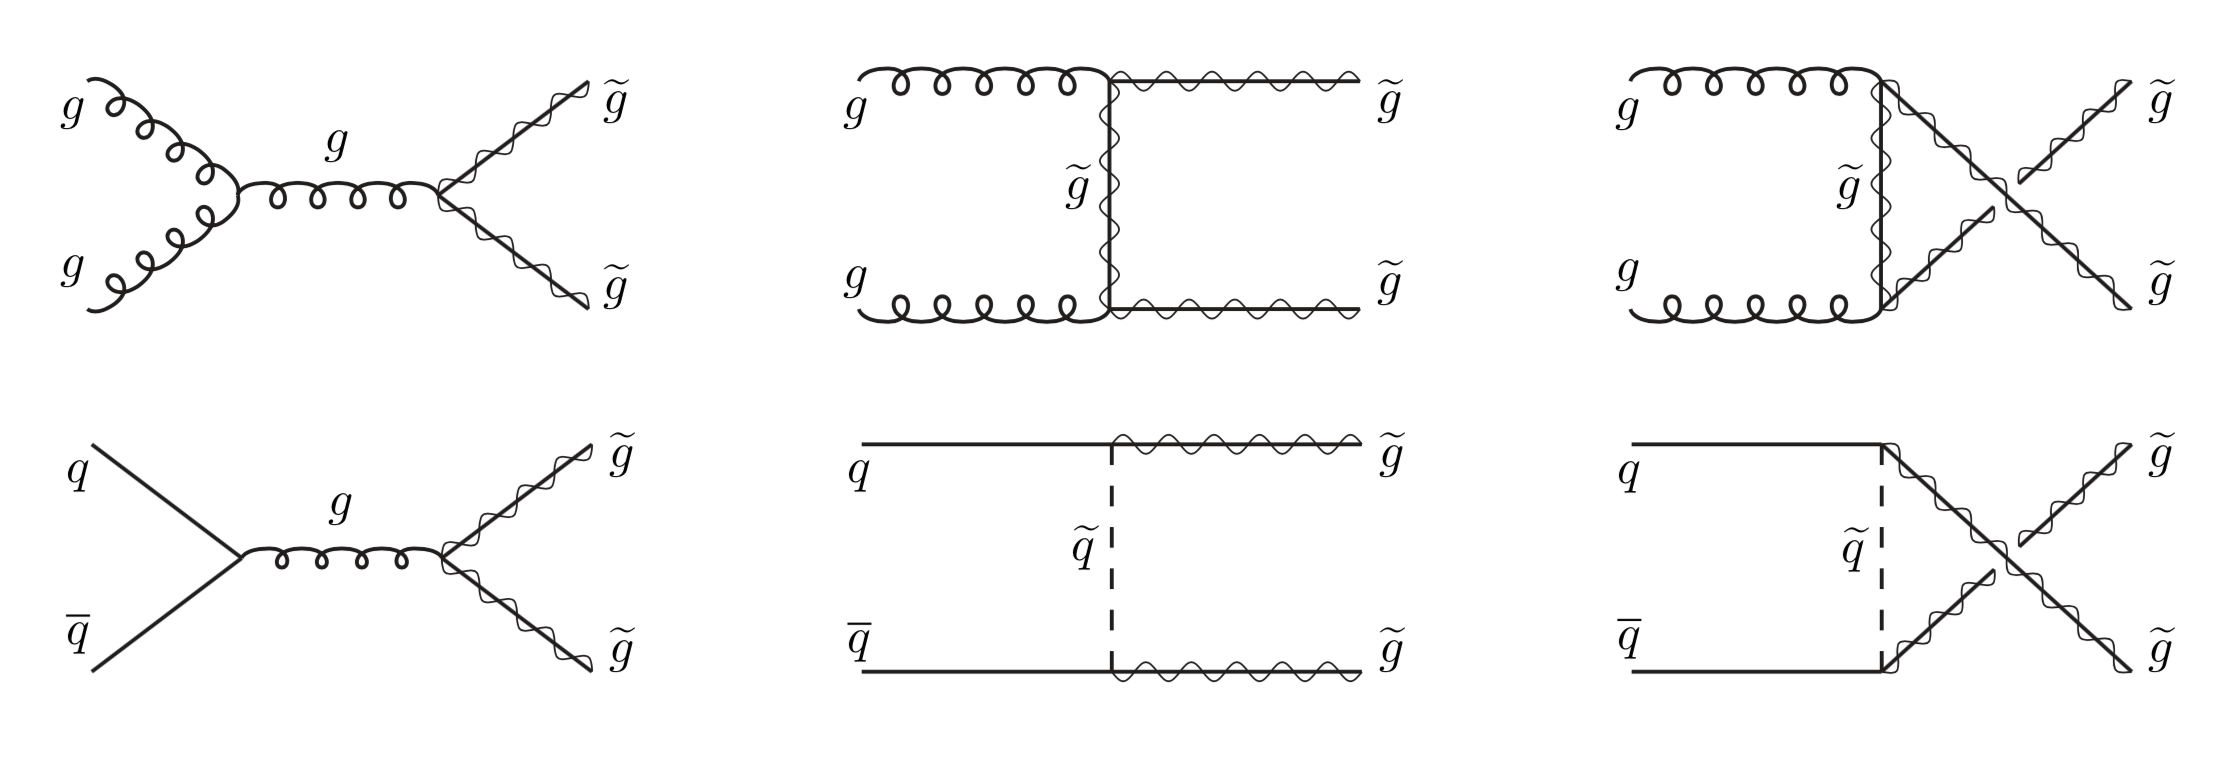
\includegraphics[width=\textwidth]{figs/gluinopair}
\caption{Tree-level gluino pair-production mechanisms.}
\label{fig:gluinopair}
\end{figure}
